%%%%%%%%%%%%%%%%%%%%%%%%%%%%%%%%%%%%%%%%%%%%%%%%%%%%%%%%%%%%%%%%%%%%%%%%%%%%%%%%
%% 实验报告模板.tex                                              %%
%% author: hxp<hxp201406@gmail.com>                           %%
%% 按照基础物理实验老师发的模板更改形成                                       %%
%%%%%%%%%%%%%%%%%%%%%%%%%%%%%%%%%%%%%%%%%%%%%%%%%%%%%%%%%%%%%%%%%%%%%%%%%%%%%%%%
%% 备注:刚刚的注释刚好是80行,编写代码的时候不要超过80行,就是你的代码不要超 %%
%% 过我注释里面最后面的“%”,超过请换行。                                    %%
%%%%%%%%%%%%%%%%%%%%%%%%%%%%%%%%%%%%%%%%%%%%%%%%%%%%%%%%%%%%%%%%%%%%%%%%%%%%%%%%
%% 模板现在开始,请根据注释把相应的位置更改成对应的内容                       %%
%%%%%%%%%%%%%%%%%%%%%%%%%%%%%%%%%%%%%%%%%%%%%%%%%%%%%%%%%%%%%%%%%%%%%%%%%%%%%%%%


\documentclass{ctexart}

\usepackage{ctex}
\usepackage{amsmath}
\usepackage{amsfonts}
\usepackage{amssymb}
\usepackage{wasysym}
\newcommand{\angstrom}{\text{\normalfont\AA}}  % 定义了原子物理的A
\usepackage{graphicx}
\usepackage{float}
\restylefloat{table}
\usepackage{geometry}
\geometry{a4paper,scale=0.8}  % 定义页面大小是A4,缩放是0.8
\usepackage{caption}
\usepackage{subcaption}
\usepackage{enumitem}
\usepackage{pdfpages}

\newcommand*{\md}{\mathop{}\!\mathrm{d}}   % 定义微分算子,直立体的d
\newcommand*{\me}{\mathrm{e}}              % 定义自然对数e,同样应当是直立体

% 如果你想要每一段的开头不要空两格,注释掉下面这两行
\usepackage{parskip}
\setlength{\parindent}{0cm}

% 默认的\mathbf对希腊字母不生效,这里改下
\usepackage{bm}
\let\Oldmathbf\mathbf
\renewcommand{\mathbf}[1]{\boldsymbol{\Oldmathbf{#1}}}

% 表格默认格内内容和边框没有留出距离,显示分数的时候,分数的上下会贴到边框上
% 因此我增加了表格内容和边框的最短距离是5像素
\usepackage{cellspace}
\setlength{\cellspacetoplimit}{5pt}
\setlength{\cellspacebottomlimit}{5pt}

% \si命令是用来写单位的,单位需要和之前的数字有一个空格的距离,而且应当直立体
% 用法:5 \si{km/h}
\newcommand{\si}[1]{\  \mathrm{#1}}

% 日期不要显示
\date{}

\usepackage{fancyhdr}
\pagestyle{fancy}
\fancyhf{}
\lhead{本文档TeX源码地址:https://github.com/hxp-plus/Notes/tree/master/Physics-Experiment/实验报告}
\rfoot{第 \thepage 页}
\renewcommand{\headrulewidth}{1pt}
\renewcommand{\footrulewidth}{1pt}

%% 标题三号黑体,作者信息为班级姓名学号
\newcommand{\generatetitle}[6]{\title{\zihao{3}\heiti#1} \author{#2 \quad
    \quad #3 \quad\quad #4 \quad\quad #5 \quad\quad #6} \maketitle\thispagestyle{fancy}}

%% 所有的引言、实验内容与数据处理啥的,用section
\ctexset {
  section = {
    format = \raggedright\zihao{4}\heiti,  % 设置所有section的字号为四号黑体左对齐
    name={,、},                            % 序号后跟顿号
    aftername={\hspace{0pt}},              % 修改序号和标题直接的间距为零
    number=\chinese{section},              % 设置序号为中文
  },
  subsection = {
    format = \raggedright\zihao{5}\heiti,  % 设置所有subsection的字号为五号黑体左对齐
    number={},              % 设置序号为没有序号
  },
  subsubsection = {
    format = \raggedright\zihao{5}\heiti,  % 设置所有subsection的字号为五号黑体左对齐
    number={},              % 设置序号为没有序号
  }
}

%% 实验背景、实验目的啥的,用subsection
\ctexset {
  subsection = {
    format = \raggedright\zihao{5}\heiti,  % 所有subsection的字号为五号黑体左对齐
    number={},                             % 设置序号为没有序号
  }
}

%% 把subsection之间加上中括号
\let\oldsubsection\subsection
\renewcommand{\subsection}[1]{\oldsubsection{\!\!\!\!\!\!【#1】}}
\let\oldsubsubsection\subsubsection
\renewcommand{\subsubsection}[1]{\oldsubsubsection{\!\!\!\!\!\!【#1】}}

%% 摘要和关键词用paragraph

\ctexset {
  paragraph = {
    format = \raggedright\zihao{5}\heiti,  % 所有paragraph的字号为五号黑体左对齐
    number={},                             % 设置序号为没有序号
  }
}

%% 把paragraph之间加上中括号
\let\oldparagraph\paragraph
\renewcommand{\paragraph}[1]{\oldparagraph{#1:\!\!\!\!\!\!}}

%% 再把参考文献的序号去掉
\makeatletter
\renewcommand\@biblabel[1]{}
\makeatother

\begin{document}

\generatetitle{综合物理实验报告——
  分光计的调整与使用}{物理4+4}{胡喜平}{U201811966}{hxp201406@gmail.com}{https://hxp.plus/}

\paragraph{摘要}
本次实验认识并使用的分光计,熟悉分光计的工作原理,并掌握分光计的光路调节。之后用分光计进行三棱镜的顶角测量、观察三棱镜和衍射光栅分开的汞灯光谱,并进行相关测量。

% 关键词
\paragraph{关键词}
分光计、光栅、三棱镜

\section{实验原理}

\subsection{分光计的原理}

这是分光计的示意图,左边是平行光管,右边是自准直望远镜。

\begin{figure}[H]
  \centering
  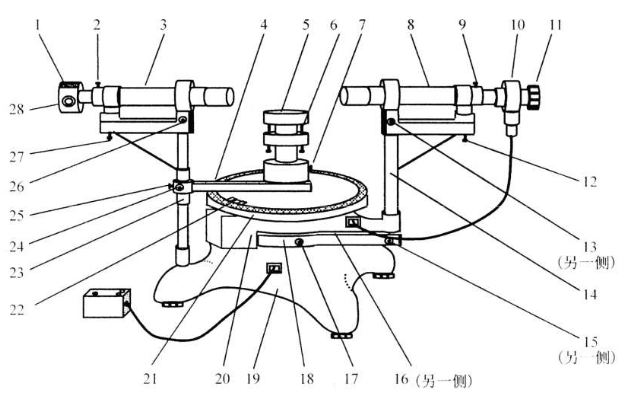
\includegraphics[width=\linewidth]{figures/分光计示意图}
  \caption{分光计示意图}
  \label{fig:分光计示意图}
\end{figure}

\begin{figure}[H]
  \centering
  \begin{subfigure}{.35\textwidth}
    \centering
    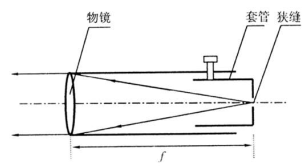
\includegraphics[width=\linewidth]{figures/平行光管示意图}
    \caption{平行光管示意图}
  \end{subfigure}
  \begin{subfigure}{.6\textwidth}
    \centering
    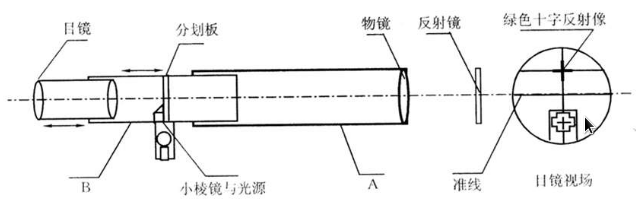
\includegraphics[width=\linewidth]{figures/自准直望远镜示意图}
    \caption{自准直望远镜示意图}
  \end{subfigure}
\end{figure}

平行光管用来产生平行光,自准直望远镜用来观察平行光。分光计中平行光管不可转动,望远镜支架可以转动,载物台可以转动。其中有一个螺丝控制载物台是否和内盘的游标一起转动。

读数装置和游标卡尺相似,外盘是主刻度,内盘有游标。分光计有两套游标,读取角度的时候分别记录两个游标,之后取平均值。

\subsection{望远镜的调节}

首先调节目镜使在目镜中能看见清晰的准线,之后不要动目镜,打开望远镜的照明灯,手持平面镜贴近望远镜物镜,移动镜筒B来调整分划板的位置,直到反射回来的绿色十字在分划板准线上,且反射回来的像最清晰,且像不会随着观察者的位置变化而改变。

之后调节望远镜和旋转中心轴垂直,将反射镜放置在载物台上,如果不垂直,那么反射镜旋转半周后,目镜中观察到的绿色十字位置会改变,这时候调节望远镜的角度使得十字位置回去一半,再调节载物台的角度使得十字位置回去另一半,再让反射镜旋转半周,重复操作,直到旋转半周以后十字的位置不发生改变。

\begin{figure}[H]
  \centering
  \begin{subfigure}{.3\textwidth}
    \centering
    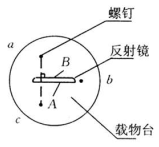
\includegraphics[width=\linewidth]{figures/在载物台上放置反射镜}
    \caption{在载物台上放置反射镜}
  \end{subfigure}
  \begin{subfigure}{.6\textwidth}
    \centering
    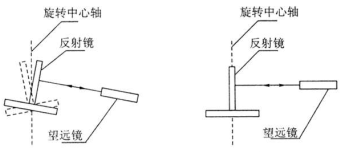
\includegraphics[width=\linewidth]{figures/调节望远镜和旋转中心轴垂直}
    \caption{调节望远镜和旋转中心轴垂直}
  \end{subfigure}
\end{figure}

\subsection{平行光管的调节}

先调节到大致平行的状态上,让平行光管发出的光能大致平行地进入望远镜。之后调节狭缝的前后位置,使得望远镜目镜上有清晰的、不随观察者位置改变的像。

之后仔细调整平行光管的俯仰角度使得狭缝的像在望远镜中正好与准线的中心重合。旋转狭缝半周,继续调节平行光管的俯仰角度,使得狭缝的像与准线中心重合,重复几次直到旋转后不需要调节俯仰角就已经重合。

\subsection{三棱镜的调节}

  如下图所示,将三棱镜放在载物台上,使得三棱镜的三边与载物台上三个螺丝的连线垂直。三棱镜的BC面为毛玻璃,先让AC面垂直于望远镜,开望远镜电源,调节螺丝a使得绿色十字在准线交点,再对AB做同样操作。

\begin{figure}[H]
  \centering
  \begin{subfigure}{.25\textwidth}
    \centering
    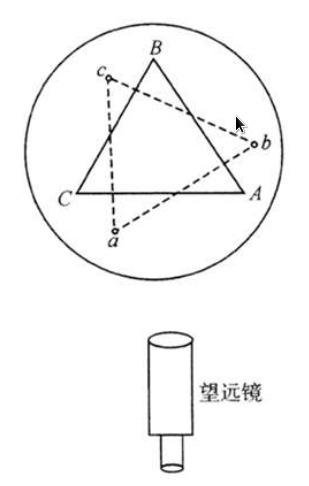
\includegraphics[width=\linewidth]{figures/三棱镜的调节}
    \caption{三棱镜的调节}
  \end{subfigure}
  \begin{subfigure}{.7\textwidth}
    \centering
    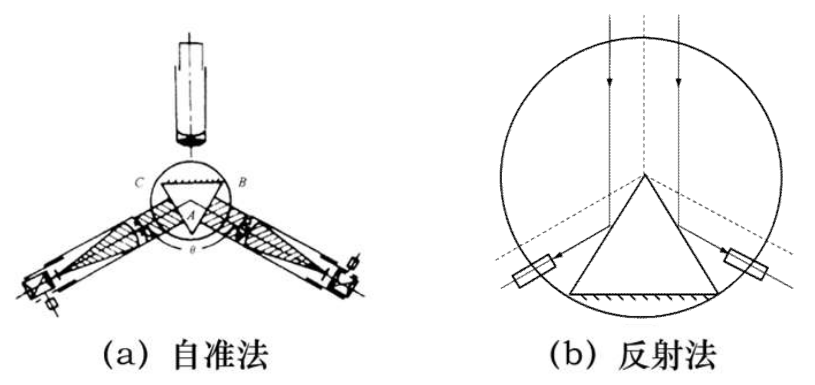
\includegraphics[width=\linewidth]{figures/三棱镜顶角的测量}
    \caption{测量三棱镜的顶角}
  \end{subfigure}
\end{figure}

\subsection{测量三棱镜的顶角}

测量三棱镜顶角的两种方法如上图所示。如果使用自准法,旋转望远镜使得望远镜在$\varphi_1$和$\varphi_2$两个角度时,望远镜上的十字和准线重合,则顶角为

\begin{equation*}
  \begin{aligned}
    \alpha = \pi - \left| \varphi_1 - \varphi_2 \right|
  \end{aligned}
\end{equation*}

如果使用反射法,打开平行光源,旋转望远镜,使得望远镜中准线交点和光源重合的角度分别为$\varphi_1$和$\varphi_2$,顶角为

\begin{equation*}
  \begin{aligned}
    \alpha = \dfrac{1}{2}  \left| \varphi_1 - \varphi_2 \right|
  \end{aligned}
\end{equation*}

\subsection{观察汞灯光谱并测量谱线的折射率}

测量折射率的时候先旋转三棱镜到最小偏向角,之后转动望远镜使得谱线在准线交点,记录当前角度$\varphi_1$,之后拿掉三棱镜让光源直接打到望远镜准线交点上,记录当前角度$\varphi_2$,则最小偏向角为

\begin{equation*}
  \begin{aligned}
    \delta_{min} = \left| \varphi_1 - \varphi_2 \right|
  \end{aligned}
\end{equation*}

三棱镜的最小偏向角$\delta_{min}$和折射率$n$以及顶角$\alpha$的关系为

\begin{equation*}
  \begin{aligned}
    n = \dfrac{\sin \left[ \left( \alpha + \delta_{min} \right)/2 \right]}{\sin \left( \alpha /2 \right)} 
  \end{aligned}
\end{equation*}

用这个公式计算折射率

\begin{figure}[H]
  \centering
  \begin{subfigure}{.65\textwidth}
    \centering
    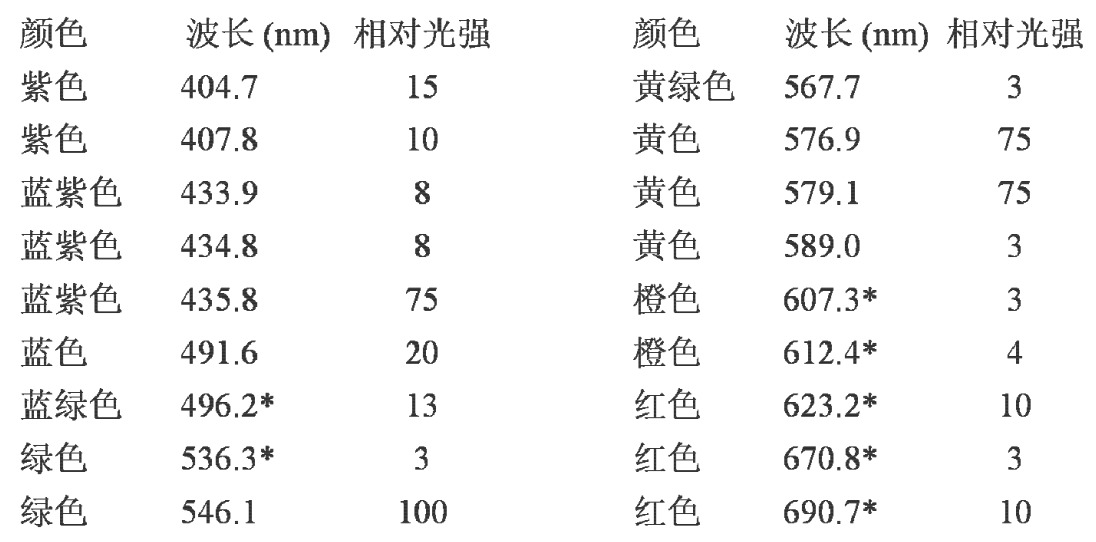
\includegraphics[width=\linewidth]{figures/汞灯光谱}
    \caption{汞灯光谱}
  \end{subfigure}
  \begin{subfigure}{.3\textwidth}
    \centering
    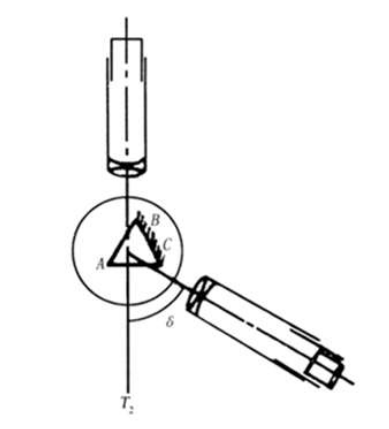
\includegraphics[width=\linewidth]{figures/三棱镜最小偏向角测量}
    \caption{三棱镜最小偏向角测量}
  \end{subfigure}
\end{figure}

\subsection{光栅常数的测量}

光栅衍射明纹条件为

\begin{equation*}
  \begin{aligned}
    d \sin \theta = k \lambda
  \end{aligned}
\end{equation*}

选择一个谱线,测量它的$\pm 1$极衍射条纹,则两次测量的角度差是$k=1$时的$2\theta$,则

\begin{equation*}
  \begin{aligned}
    d= \dfrac{2 \lambda}{\left| \varphi_1 - \varphi_2 \right|} 
  \end{aligned}
\end{equation*}

\section{实验内容}

\begin{itemize}
\item 按照分光计的调节要求和方法调节分光计
\item 测量三棱镜的顶角
\item 观察经三棱镜分光后的汞灯光谱,并测量各谱线折射率
\item 测量光栅常数
\end{itemize}

\section{实验结果的分析和结论}

所有的实验数据都是交给附录里面的程序自动处理的,此文档下面的内容均为程序自动生成,表格为程序自动填写,本人人工检查程序处理结果。
代码在https://github.com/hxp-plus/Spectrometer-Experiment也有一份拷贝。

\subsection{自准法测量三棱镜顶角数据}

用一个游标测得的数据如下:

\begin{table}[H]
  \centering
  \begin{tabular}{|c|c|c|c|c|c|}
    \hline
     测量次数           & 1 & 2 & 3 & 4 & 5 
     \\\hline
     转动前的角度 &$77^\circ 33^\prime$&$77^\circ 33^\prime$&$77^\circ 33^\prime$&$77^\circ 33^\prime$&$77^\circ 33^\prime$\\\hline
     转动后的角度 &$197^\circ 35^\prime$&$197^\circ 35^\prime$&$197^\circ 35^\prime$&$197^\circ 35^\prime$&$197^\circ 35^\prime$\\\hline
  \end{tabular}
  \caption{自准法测量三棱镜顶角数据}
\end{table}

计算得出转动前角度平均值为:$77.550000^\circ$ \\
计算得出转动后角度平均值为:$197.583333^\circ$ \\
进而计算得出三棱镜顶角为:$59.966667^\circ$ \\

用另一个游标测得的数据如下:

\begin{table}[H]
  \centering
  \begin{tabular}{|c|c|c|c|c|c|}
    \hline
     测量次数           & 1 & 2 & 3 & 4 & 5 \\\hline
     转动前的角度 &$257^\circ 30^\prime$&$257^\circ 30^\prime$&$257^\circ 30^\prime$&$257^\circ 34^\prime$&$257^\circ 34^\prime$\\\hline
     转动后的角度 &$17^\circ 33^\prime$&$17^\circ 35^\prime$&$17^\circ 36^\prime$&$17^\circ 36^\prime$&$17^\circ 36^\prime$\\\hline
  \end{tabular}
  \caption{自准法测量三棱镜顶角数据}
\end{table}

计算得出转动前角度平均值为:$257.526667^\circ$ \\
计算得出转动后角度平均值为:$377.586667^\circ$ \\
进而计算得出三棱镜顶角为:$59.940000^\circ$ \\
两次计算的平均顶角为:$59.953333^\circ$

\subsection{反射法测量三棱镜顶角数据}

用一个游标测得的数据如下:

\begin{table}[H]
  \centering
  \begin{tabular}{|c|c|c|c|c|c|}
    \hline
     测量次数           & 1 & 2 & 3 & 4 & 5 
     \\\hline
     转动前的角度 &$83^\circ 20^\prime$&$83^\circ 20^\prime$&$83^\circ 20^\prime$&$83^\circ 19^\prime$&$83^\circ 20^\prime$\\\hline
     转动后的角度 &$203^\circ 14^\prime$&$203^\circ 15^\prime$&$203^\circ 14^\prime$&$203^\circ 14^\prime$&$203^\circ 15^\prime$\\\hline
  \end{tabular}
  \caption{反射法测量三棱镜顶角数据}
\end{table}

计算得出转动前角度平均值为:$83.330000^\circ$ \\
计算得出转动后角度平均值为:$203.240000^\circ$ \\
进而计算得出三棱镜顶角为:$59.955000^\circ$ \\

用另一个游标测得的数据如下:

\begin{table}[H]
  \centering
  \begin{tabular}{|c|c|c|c|c|c|}
    \hline
     测量次数           & 1 & 2 & 3 & 4 & 5 \\\hline
     转动前的角度 &$263^\circ 30^\prime$&$263^\circ 18^\prime$&$263^\circ 21^\prime$&$263^\circ 18^\prime$&$263^\circ 19^\prime$\\\hline
     转动后的角度 &$23^\circ 16^\prime$&$23^\circ 15^\prime$&$23^\circ 16^\prime$&$23^\circ 16^\prime$&$23^\circ 15^\prime$\\\hline
  \end{tabular}
  \caption{反射法测量三棱镜顶角数据}
\end{table}

计算得出转动前角度平均值为:$263.353333^\circ$ \\
计算得出转动后角度平均值为:$383.260000^\circ$ \\
进而计算得出三棱镜顶角为:$59.953333^\circ$ \\
两次计算的平均顶角为:$59.954167^\circ$

\subsection{测量最小偏向角}

实验中三棱镜顶角取上面所有数据的平均值 $59.953750^\circ$

其中$\theta_1$和$\theta_2$是放置棱镜时,两个游标的度数。$\theta_1‘$和$\theta_2’$是不放置棱镜时,两个游标的度数。$\Delta \theta$是偏转角,$n$是计算得到的折射率。

\begin{table}[H]
  \centering
  \begin{tabular}{|c|c|c|c|c|c|c|}
    \hline
     波长(nm) & $\theta_1$ & $\theta_2$ & $\theta_1'$ & $\theta_2'$ & $\Delta \theta$ & $n$\\\hline
    407.0&$200^\circ17^\prime$ &$20^\circ19^\prime$ &$138^\circ23^\prime$ &$318^\circ23^\prime$ &$61.916667^\circ$ &$1.749365$\\\hline
    546.0&$197^\circ18^\prime$ &$17^\circ21^\prime$ &$138^\circ23^\prime$ &$318^\circ23^\prime$ &$58.941667^\circ$ &$1.723536$\\\hline
    578.0&$196^\circ50^\prime$ &$16^\circ49^\prime$ &$138^\circ23^\prime$ &$318^\circ23^\prime$ &$58.441667^\circ$ &$1.719081$\\\hline
    589.0&$196^\circ48^\prime$ &$16^\circ48^\prime$ &$138^\circ23^\prime$ &$318^\circ23^\prime$ &$58.416667^\circ$ &$1.718857$\\\hline
  \end{tabular}
  \caption{测量最小偏向角}
\end{table}


\subsection{测量光栅常数}

$\theta_{+1}$和$\theta_{+1}'$是条纹在$+1$级时,两个游标的读数。$\theta_0$和$\theta_0'$是条纹在$0$级时,两个游标的读数。$\theta_{-1}$和$\theta_{-1}'$是条纹在$-1$级时,两个游标的读数。

\begin{table}[H]
  \centering
  \begin{tabular}{|c|c|c|c|c|c|c|c|c|}
    \hline
     波长(nm) &  $\theta_{+1}$ & $\theta_{+1}'$ & $\theta_0$ & $\theta_0'$ & $\theta_{-1}$ & $\theta_{-1}'$ & $\Delta \theta$ & 光栅常数(nm)\\\hline
    407.0&$153^\circ1^\prime$ &$333^\circ0^\prime$ &$138^\circ22^\prime$ &$318^\circ22^\prime$ &$123^\circ12^\prime$ &$303^\circ12^\prime$ &$14.904167^\circ$ &$1582.407244$\\\hline
    546.0&$157^\circ30^\prime$ &$337^\circ30^\prime$ &$138^\circ22^\prime$ &$318^\circ22^\prime$ &$119^\circ12^\prime$ &$299^\circ12^\prime$ &$19.150000^\circ$ &$1664.419001$\\\hline
    578.0&$158^\circ5^\prime$ &$338^\circ5^\prime$ &$138^\circ22^\prime$ &$318^\circ22^\prime$ &$118^\circ4^\prime$ &$298^\circ5^\prime$ &$20.004167^\circ$ &$1689.621358$\\\hline
    589.0&$158^\circ41^\prime$ &$338^\circ39^\prime$ &$138^\circ22^\prime$ &$318^\circ22^\prime$ &$118^\circ0^\prime$ &$298^\circ0^\prime$ &$20.333333^\circ$ &$1695.055564$\\\hline
  \end{tabular}
  \caption{测量光栅常数}
\end{table}

\section{参考文献}

\begin{itemize}[leftmargin=0pt]
\item[] 综合物理实验讲义
\end{itemize}

\section{附录:处理并自动生成并填写此实验报告表格的程序}

程序GitHub仓库在https://github.com/hxp-plus/Spectrometer-Experiment,背面是程序的所有文件以及程序处理时读取的数据文件

\includepdf[pages={1-},angle=0]{分光计的调整与使用/分光计的调整与使用源代码.pdf}

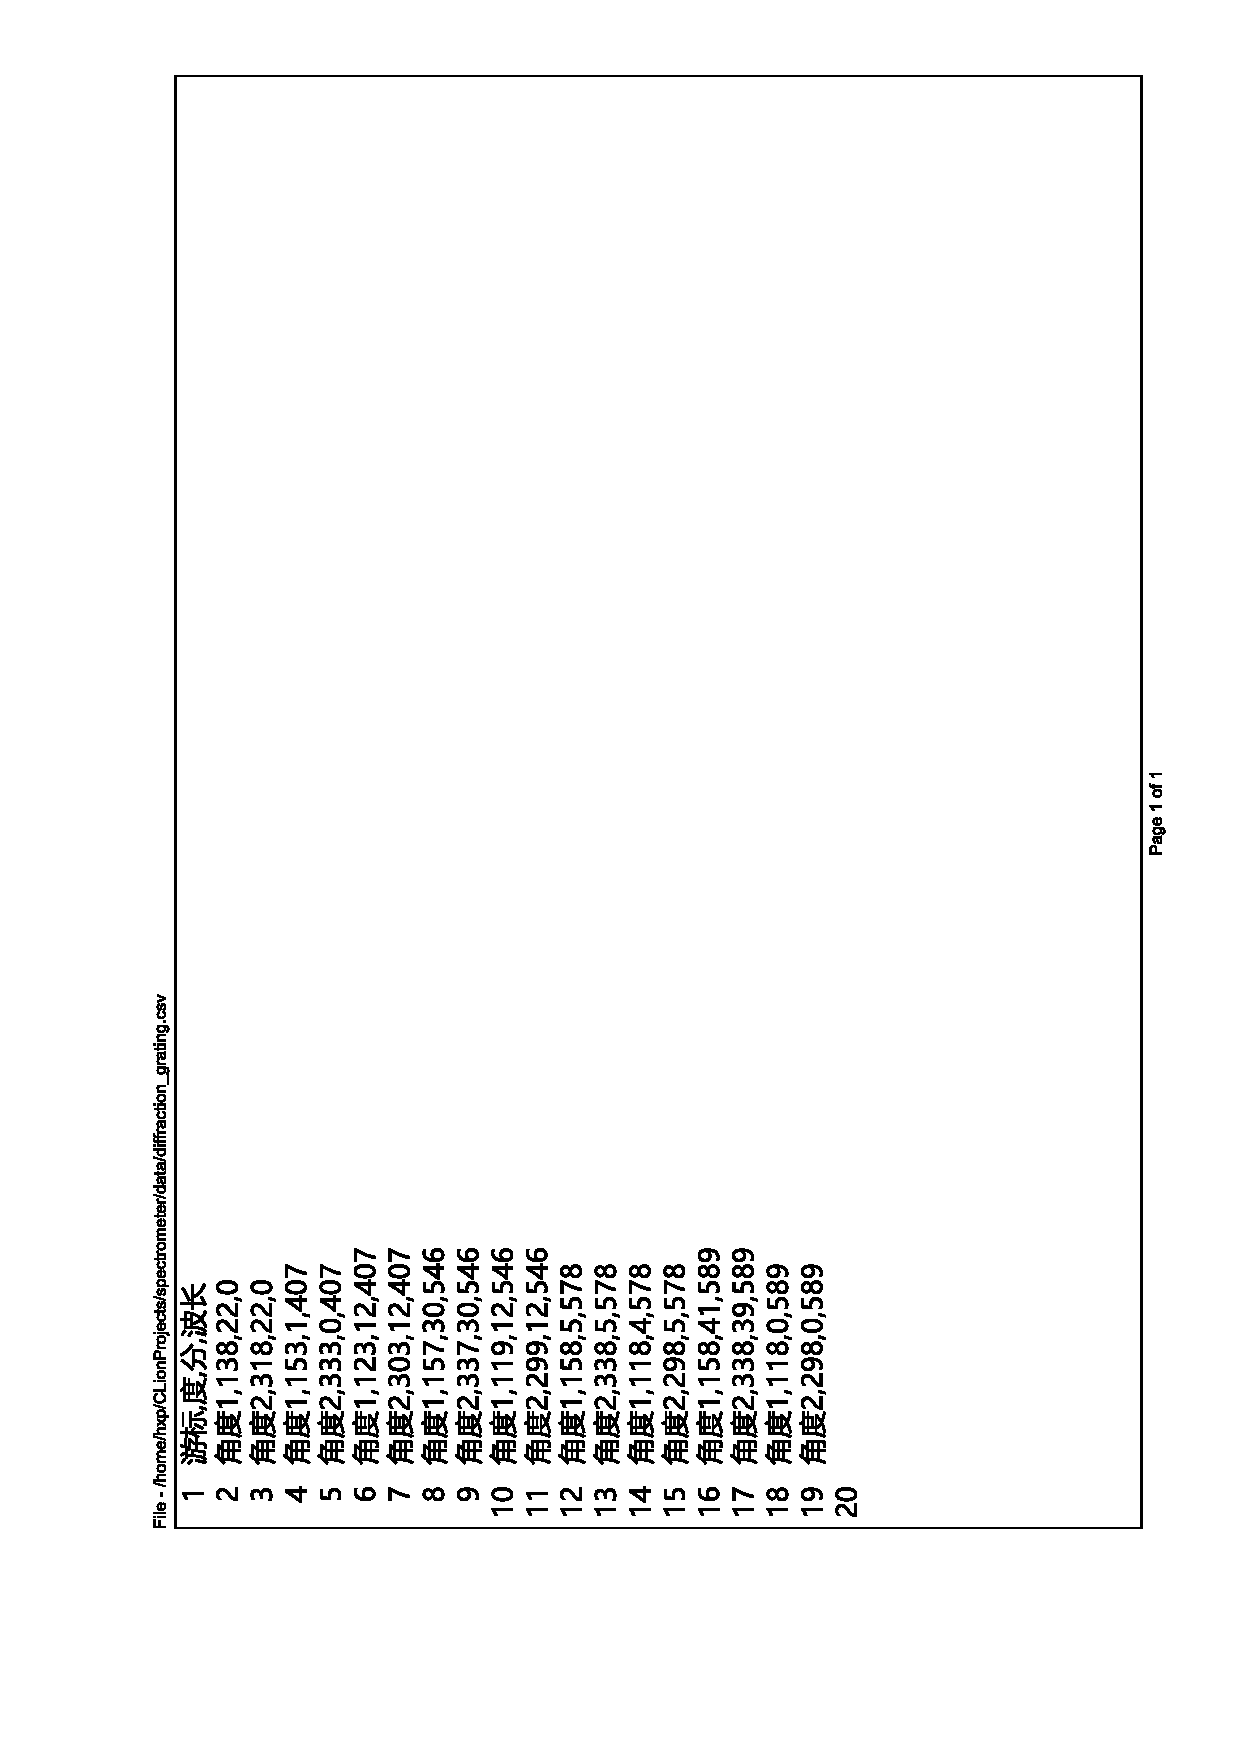
\includepdf[pages={1-},angle=0]{分光计的调整与使用/分光计的调整与使用数据.pdf}

\end{document} 
